\subsection{Introduction}
\begin{frame}[containsverbatim]
\frametitle{Parallelization mini-projects}

\begin{itemize}
	\item{60 hours of personal work}
	\item{Individual (for some hard problems : binom)}
	\item{We propose subjects but \textbf{you can propose yours !}}
	\item{MPI or CUDA (OpenMP/hybrid/MPI-IO are a plus)}
\end{itemize}

%\begin{alertblock}{Blabla}
%\begin{alertblock}{Blabla}
%\begin{block}{Blabla}
%\end{block}

Important dates :

\begin{center}
\begin{tabular}{ | l | l |}
\hline
\textbf{Deliverable} & \textbf{Due date} \\
\hline
Fixing topic & May 2, 2016 \\
\hline
Theoretical Analysis & May 15, 2016 \\
\hline
Final Report & June 5, 2016 \\
\hline
Exam (15' pres + 15' Q\&A) & June 23, 2016 8:15-18:00 \\
&and June 24, 2016 8:15-18:00 \\
\hline
\end{tabular}	
\end{center}

(all at 11:59 pm. CEST)

\end{frame}




\subsection{Julia set}
\begin{frame}[containsverbatim]
\frametitle{Julia set}
\begin{center}
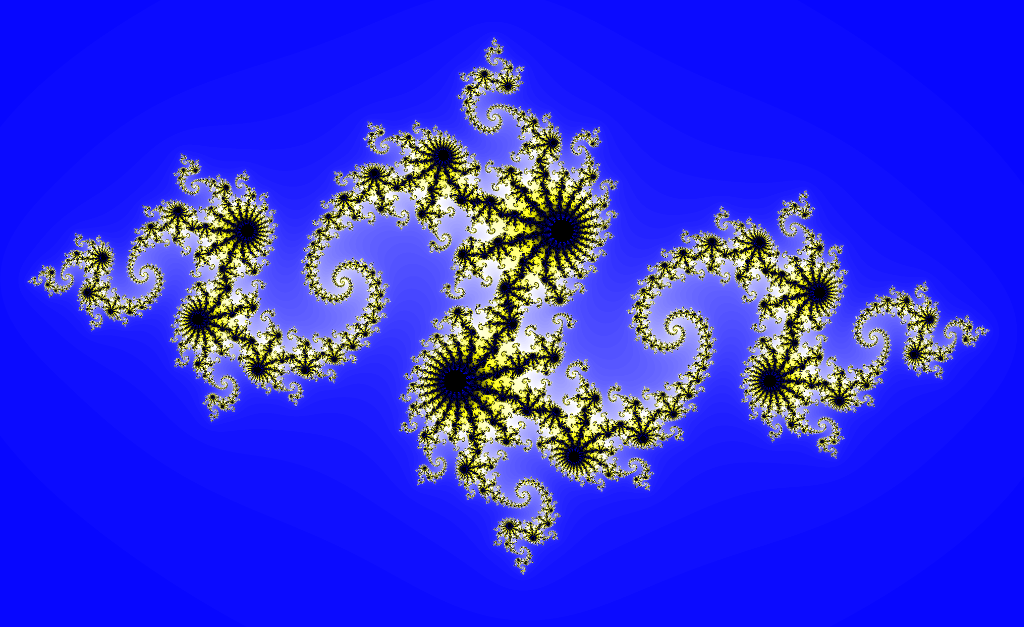
\includegraphics[width=5.0cm]{Day2/images/julia2.png}
\end{center}
\begin{block}{Problem description}
The Julia set is the set of points of the complex plan $z = a + b i$ such that the suite
$$
z_{(n+1)} = z_n^2 + c
$$
remains bounded when $n \rightarrow \infty$. $c$ is a constant. 
\end{block}
\end{frame}
\begin{frame}[containsverbatim]
\frametitle{Julia set}
\begin{block}{Important remarks}
\begin{itemize}
	\item{load balancing}
\end{itemize}
\end{block}
\end{frame}



\subsection{Mandelbrot set}
\begin{frame}[containsverbatim]
\frametitle{Mandelbrodt set}
\begin{center}

\includegraphics[width=3.0cm]{Day2/images/mandelbrot.jpg}
\end{center}
\begin{block}{Problem description}
The Mandelbrot set is the set of complex numbers $c$ obtained by the quadratic recurrence equation :
$$
\left\{ \begin{array}{r}
 z_0 = 0 \\
  z_{(n+1)} = z_n^2 + c
       \end{array} \right.
$$
such the suite does not diverge when $n \rightarrow \infty$. 
\end{block}
\end{frame}
\begin{frame}[containsverbatim]
\frametitle{Mandelbrodt set}
\begin{block}{Important remarks}
\begin{itemize}
	\item{load balancing}
	\item{a \textit{colored plot} is obtained by coloring the points with the number of steps required to reach the cut-off value $r_{max}$ value (usually $r_{max} = 2$)}
	\item{Mandelbrot set is considered as a ``map'' of all the Julia sets because it uses a different $c$ at each $z$.}
\end{itemize}
\end{block}
\end{frame}




\subsection{Traveling Salesman Problem}
\begin{frame}[containsverbatim]
\frametitle{Traveling Salesman Problem}
\begin{center}
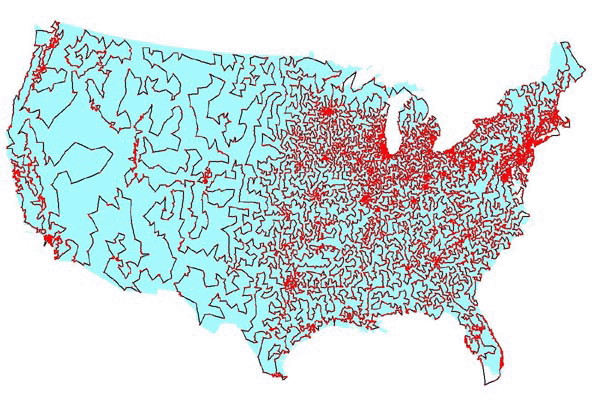
\includegraphics[width=4.0cm]{Day2/images/tsp.png}
\\
{\tiny Figure credit: David Applegate, Robert Bixby, Vasek Chvatal and William Cook.}
\end{center}
\begin{block}{Problem description}
Let us have an undirected weighted graph where : cities are the vertices, the edges are the paths, the weight a distance between two cities. The TSP solution is the shortest path starting and finishing at the same vertice and by visiting all the other vertices one and only one time.
\end{block}
\end{frame}
\begin{frame}[containsverbatim]
\frametitle{Traveling Salesman Problem}
\begin{block}{Important remarks}
\begin{itemize}
	\item{load balancing}
	\item{tree construction}
\end{itemize}
\end{block}
\end{frame}




\subsection{N-queens problem}
\begin{frame}[containsverbatim]
\frametitle{N queens problem}
\begin{center}

\includegraphics[width=4.0cm]{Day2/images/queen.jpg}
\end{center}
\begin{block}{Problem description}
The N-queens problem is the problem of placing $N$ queens on an $N \times N$ board ($N>3$) so that no queen see each other. A queen can move on its row, its column and its diagonals.
\end{block}
\end{frame}
%\begin{frame}[containsverbatim]
%\frametitle{n queens problem}
%\begin{block}{Important remarks}
%\begin{itemize}
%	\item{tree construction}
%	\item{}
%\end{itemize}
%\end{block}
%\end{frame}




\subsection{FFT}
\begin{frame}[containsverbatim]
\frametitle{FFT with Cooley-Tukey}
\begin{center}
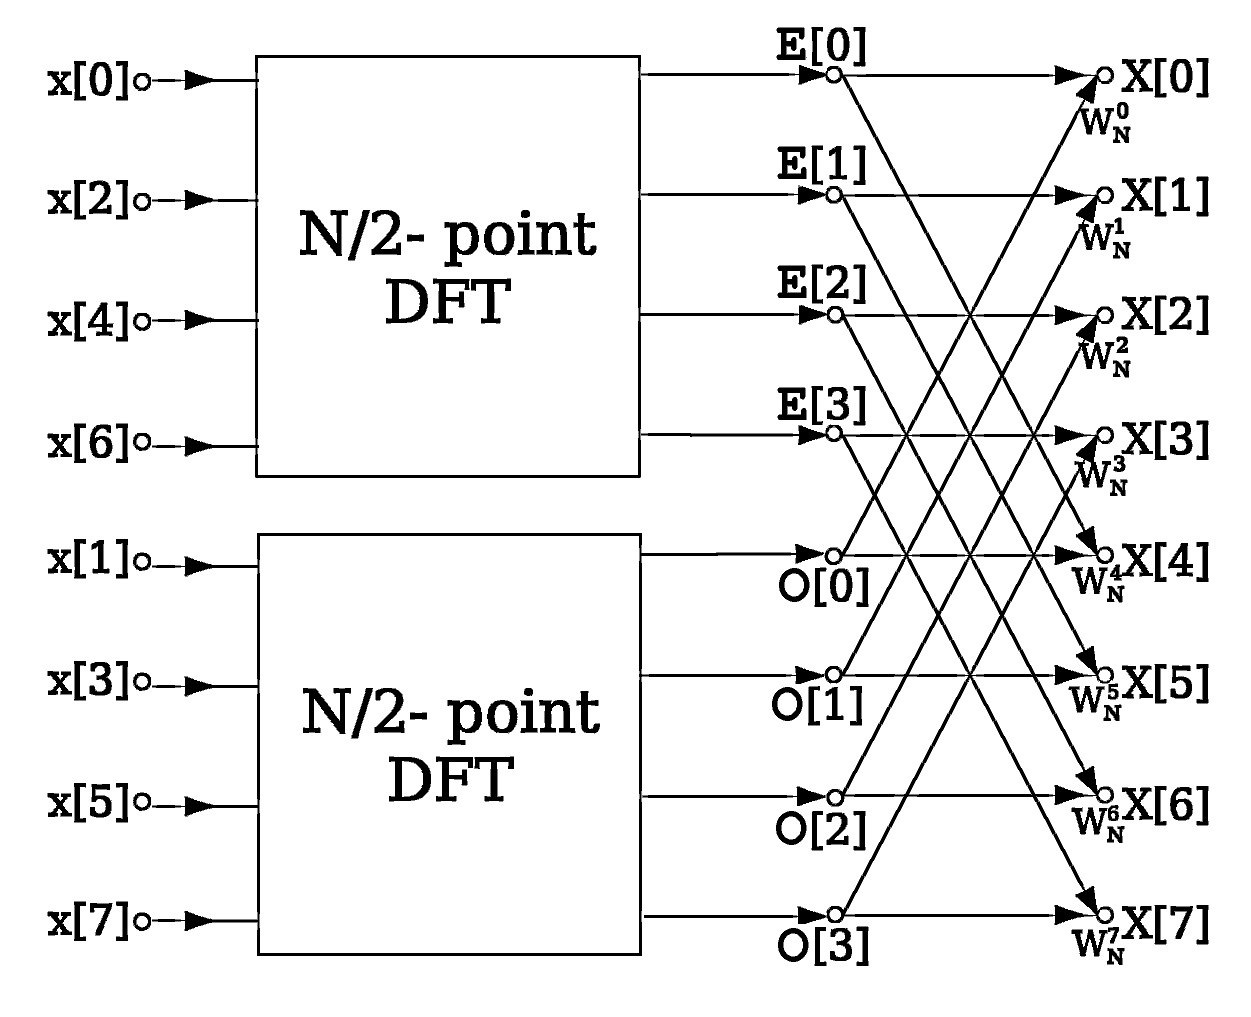
\includegraphics[width=4.0cm]{Day2/images/fft.png}
\end{center}
\begin{block}{Problem description}
The Fast Fourier Transform (FFT) Cooley-Tukey algorithm computes the Discrete Fourier Transform (DFT) of a sequence recursively by a devide-and-conquer approach. The radix-2 decimation in time divides a DFT of size $N$ into two interleaved DFT of size $N/2$.
\end{block}
\end{frame}
%\begin{frame}[containsverbatim]
%\frametitle{FFT with Cooley-Tukey}
%A DFT is described as :
%$$
%X_k = \sum_{n=0}^{N-1} x_n e^{- \frac{2 \pi i}{N} n k}
%$$
%which can be rearranged as :
%$$
%X_k = \sum_{m=0}^{N/2-1} x_{2m} e^{- \frac{2 \pi i}{N/2} (2m) k} + e^{- \frac{2 \pi i}{N} k} \sum_{m=0}^{N/2-1} x_{2m+1} e^{- \frac{2 \pi i}{N/2} m k}
%$$
%in other words : the even and the odd parts of $X_k$ :
%$$
%X_k = E_k + e^{- \frac{2 \pi i}{N}k} O_k
%$$
%\end{frame}
%\begin{frame}[containsverbatim]
%\frametitle{FFT with Cooley-Tukey}
%Therefore:
%$$
%X_k = \left\{ \begin{array}{ll}
% E_k + e^{- \frac{2 \pi i}{N/2}k} O_k & \text{for}~~ 0 \leq k < N/2\\
%  E_{k-N/2} + e^{- \frac{2 \pi i}{N/2}k} O_{k-N/2} &\text{for}~~ N/2 \leq k < N.
%       \end{array} \right.
%$$
%we also know that :
%$$
%e^{- \frac{2 \pi i}{N}(k+ N/2)} = - e^{- \frac{2 \pi i}{N}k}
%$$
%thus for $0 \leq k < \frac{N}{2}$ :
%$$
%\begin{array}{ll}
%X_k & = E_k + e^{- \frac{2 \pi i}{N}k} O_k \\
%X_{k+\frac{N}{2}} & = E_k - e^{- \frac{2 \pi i}{N}k} O_k
%\end{array}
%$$
%\end{frame}
%\begin{frame}[containsverbatim]
%\frametitle{FFT with Cooley-Tukey}
%The DFT of length $N$ is then described in terms of two DFT of size $\frac{N}{2}$. The same process is applied recursively until $N=2$.
%\end{frame}
\begin{frame}[containsverbatim]
\frametitle{FFT with Cooley-Tukey}
\begin{block}{Important remarks}
\begin{itemize}
	\item{Complexity !}
	\item{$x_k$ reordering before devide-and-conquer}
	\item{Large size numbers $N = 2^t$ with $t$ as ``large'' as possible}
	\item{You can choose other algorithms than Cooley-Tukey}
\end{itemize}
\end{block}
\end{frame}




\subsection{Minimum spanning tree}
\begin{frame}[containsverbatim]
\frametitle{Minimum Spanning Tree}
\begin{center}
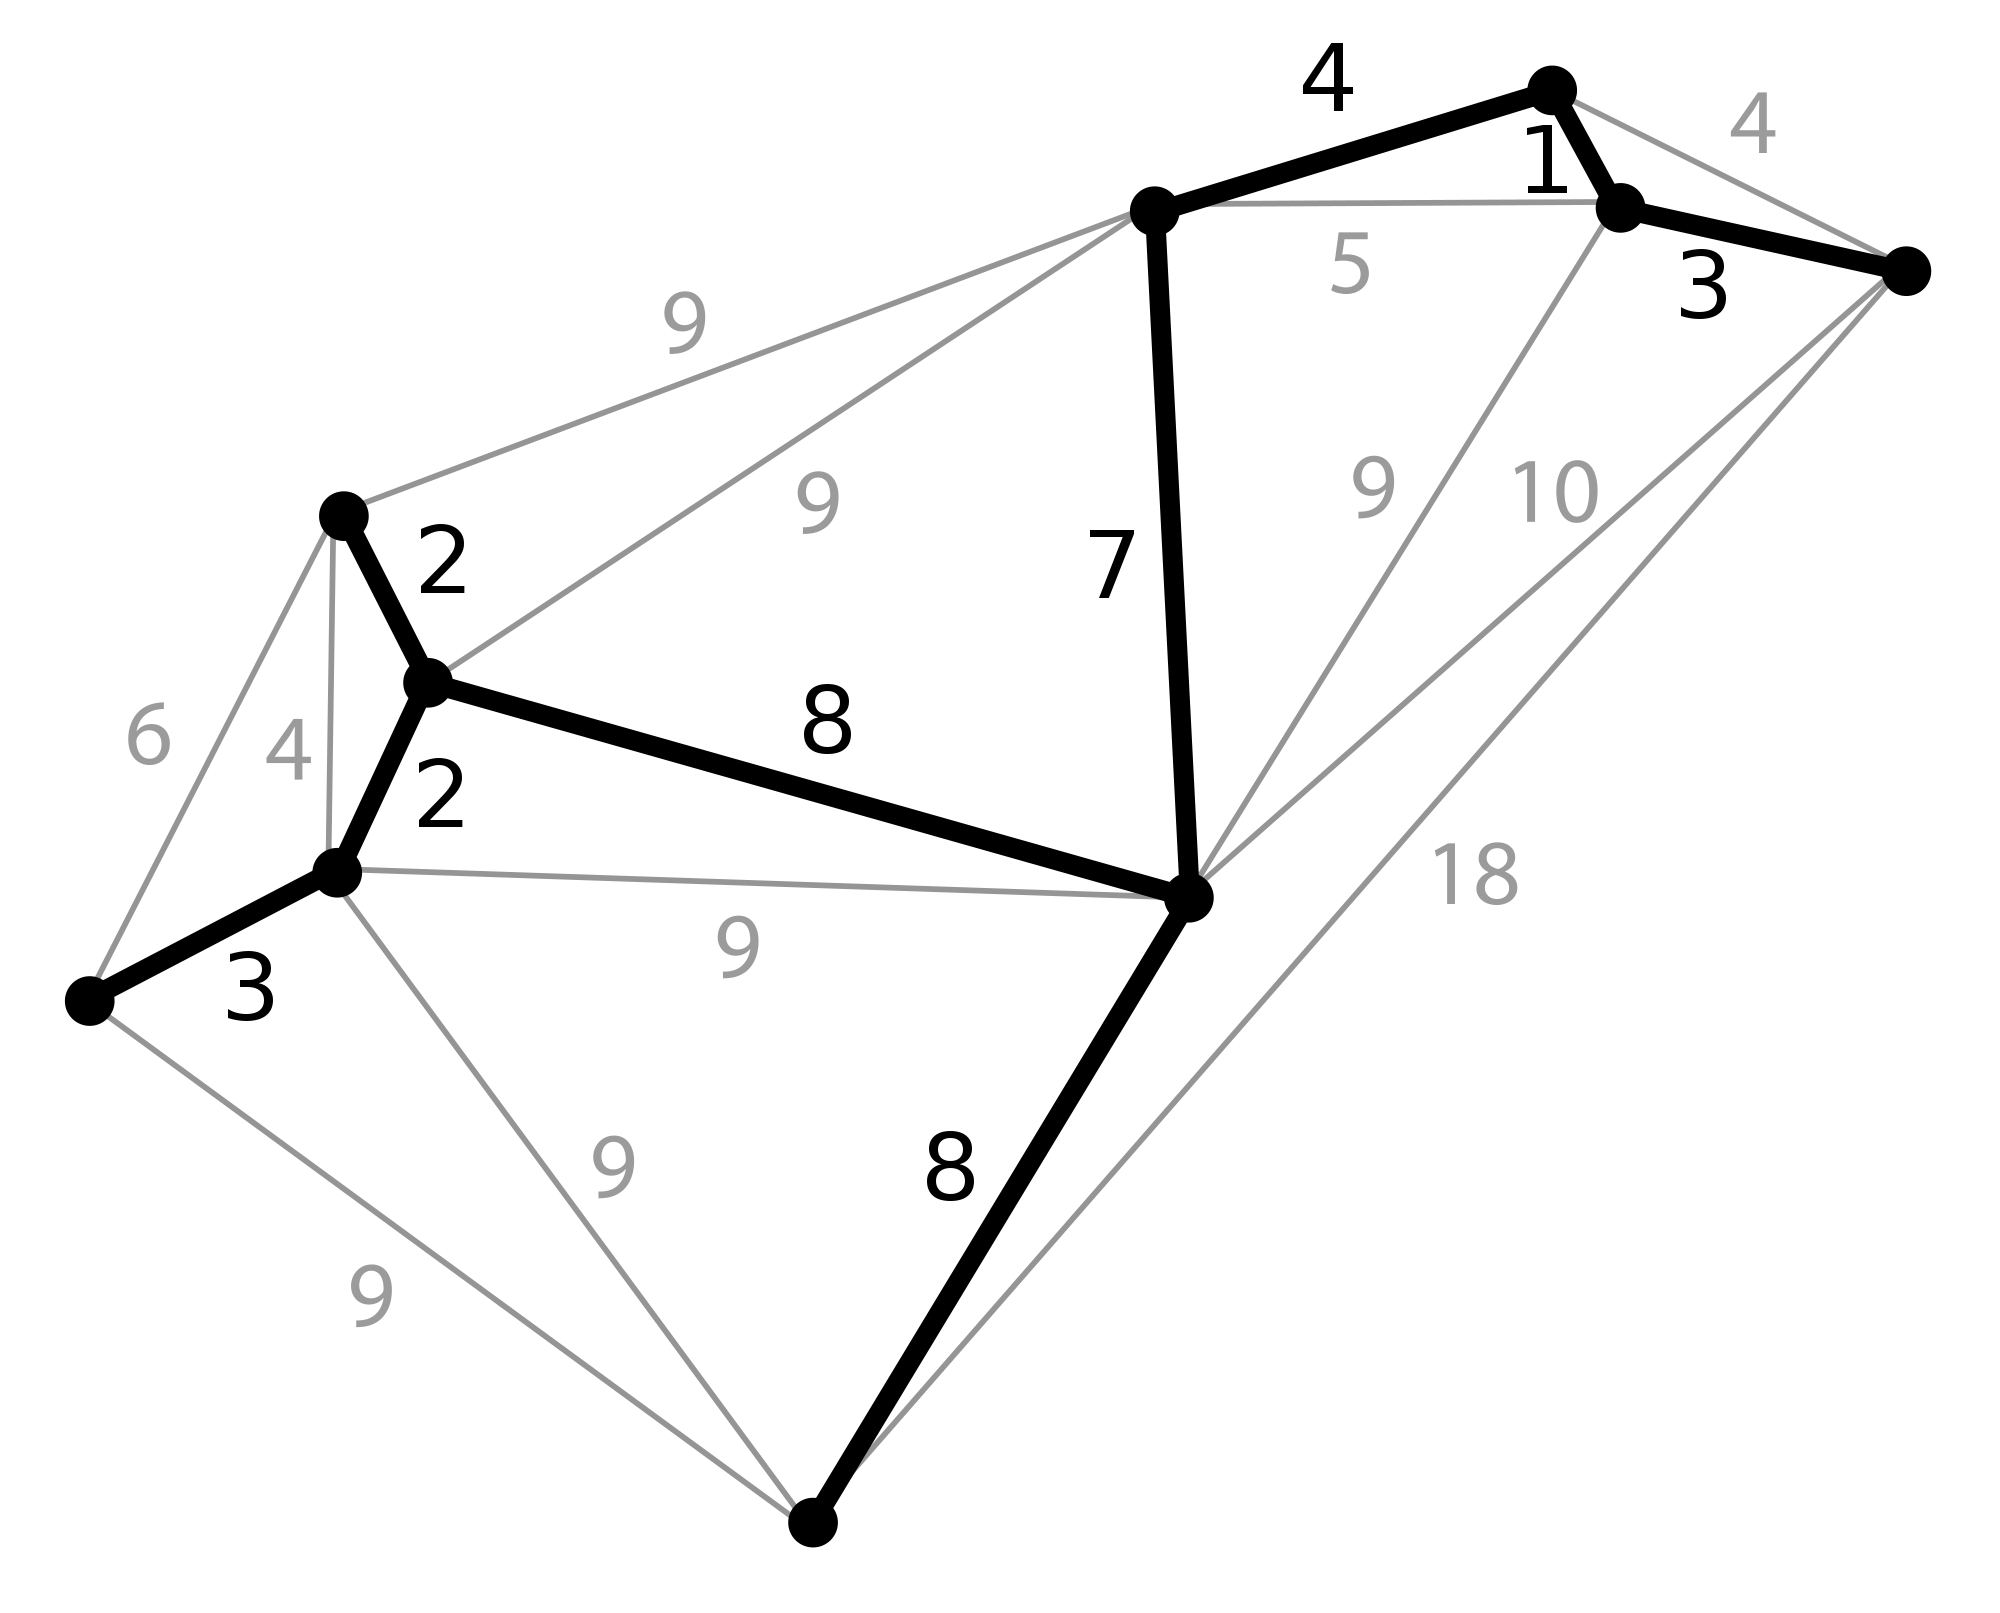
\includegraphics[width=4.0cm]{Day2/images/spanning.png}
\end{center}
\begin{block}{Problem description}
A minimum spanning tree is a spanning tree of a connected, undirected and weighted graph. It connects all the vertices together with the minimal total weighting for its edges
\end{block}
\end{frame}
\begin{frame}[containsverbatim]
\frametitle{Minimum Spanning Tree}
\begin{block}{Important remarks}
\begin{itemize}
	\item{Parallelize Boruka's algorithm}
	\item{Complexity !}
\end{itemize}
\end{block}
\end{frame}




\subsection{Dijkstra's algorithm}
\begin{frame}[containsverbatim]
\frametitle{Dijkstra's algorithm}
\begin{center}
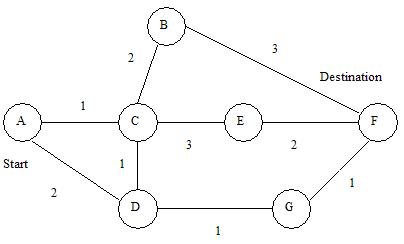
\includegraphics[width=4.0cm]{Day2/images/dijkstras.png}
\end{center}
\begin{block}{Problem description}
Dijkstra's algorithm is an algorithm for finding the shortest paths between nodes in a graph. It can be used for finding the shortest paths from a single node to a single destination node by stopping the algorithm once the shortest path to the destination node has been determined
\end{block}
\end{frame}
%\begin{frame}[containsverbatim]
%\frametitle{Dijkstra's algorithm}
%\begin{block}{Important remarks}
%\begin{itemize}
%	\item{parallelization of the tree}
%\end{itemize}
%\end{block}
%\end{frame}





\subsection{N-body simulation}
\begin{frame}[containsverbatim]
\frametitle{N-body simulation}
\begin{center}
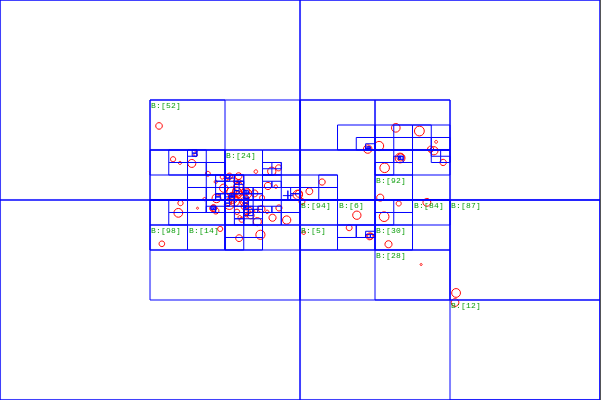
\includegraphics[width=3.0cm]{Day2/images/nbody.png}
\end{center}
\begin{block}{Problem description}
The n-body problem aims at simulating a dynamical system of particles under the influence of physical forces. We'll restrain on the gravity field applied on celestial bodies:
$$
F_{ij} = \frac{G m_i m_j (q_j - q_i)}{||q_j - q_i||}
$$
where $G$ is the gravitational constant, $m_i$ and $m_j$ the masses of the $i$-th and $j$-th bodies and $q_i$ and $q_j$ their positions.
\end{block}
\end{frame}
\begin{frame}[containsverbatim]
\frametitle{N-body simulation}
\begin{block}{Important remarks}
\begin{itemize}
	\item{brute force will not be accepted}
	\item{2D or 3D}
	\item{non-uniform initial distribution must be tested to stress the application}
	\item{how to handle collisions and ``lost bodies in the far space''}
\end{itemize}
\end{block}
\end{frame}



\subsection{Sieve of Eratosthenes}
\begin{frame}[containsverbatim]
\frametitle{Sieve of Eratosthenes}
\begin{center}
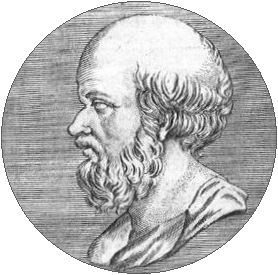
\includegraphics[width=3.0cm]{Day2/images/Eratosthene.png}
\end{center}
\begin{block}{Problem description}
Find all the prime numbers $p$ such $p < N$ where $N$ is very large. Enumerate all the multiples of $p$ by counting to $N$ in incerements of $p$ and mark them as ``non-primes''. Do that to $\sqrt{N}$. The list of $p_i$ are all the primes between $p=2$ to $p=\sqrt{N}$.
\end{block}
\end{frame}
\begin{frame}[containsverbatim]
\frametitle{Sieve of Eratosthenes}
\begin{block}{Important remarks}
\begin{itemize}
	\item{load balancing}
	\item{Handling very large numbers}
	\item{alternative : Sieve of Atkin}
\end{itemize}
\end{block}
\end{frame}





\subsection{Game of Life}
\begin{frame}[containsverbatim]
\frametitle{Game of Life}
\begin{center}
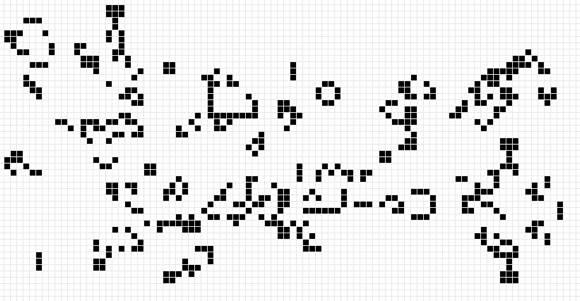
\includegraphics[width=3.0cm]{Day2/images/gameoflife.png}
\end{center}
\begin{block}{Problem description}
The game of life is a cellular automaton with simple elements: a cell $c_i$ can be dead ($c_i = 0$) or alive ($c_i = 1$). At each time step, the following rules are applied :
\begin{itemize}
	\item {if $c_i = 1$ and its neighbours are 0, 1 or 4 living cells, then $c_{i+1} = 0$}
	\item {if $c_i = 1$ and its neighbours are 2 or 3 living cells, then $c_{i+1} = 1$}
	\item {if $c_i = 0$ and its neighbours are exactly 3 living cells, then $c_{i+1} = 1$}
\end{itemize}
\end{block}
\end{frame}
\begin{frame}[containsverbatim]
\frametitle{Game of Life}
\begin{block}{Important remarks}
\begin{itemize}
	\item{as this problem is very close to Poisson, we'll accept only non-standard subdomain decomposition (topology)}
\end{itemize}
\end{block}
\end{frame}




\subsection{Jacobi iterative method}
\begin{frame}[containsverbatim]
\frametitle{Jacobi iterative method}
\begin{block}{Problem description}
The Jacobi method solves a linear system $Ax = b$ iteratively:
$$
A = D + R
$$
where D is the diagonal matrix of $A$ and $R$ the rest. The solution $x_{(k+1)}$ is obtained with:
$$
x_{(k+1)} = D^{-1} ( b - R x_k)
$$
where $x_k$ is the $k$-th iteration of $x$
\end{block}
\end{frame}



\subsection{Gauss-Seidel iterative method}
\begin{frame}[containsverbatim]
\frametitle{Gauss-Seidel iterative method}
\begin{block}{Problem description}
The Gauss-Seidel method solves a linear system $Ax = b$ iteratively:
$$
A = L + U
$$
where $L$ is the lower triangular elements of $A$ and $U$ the strict upper elements of $A$. The solution $x_{(k+1)}$ is obtained with:
$$
x_{(k+1)} = L^{-1} ( b - U x_k)
$$
where $x_k$ is the $k$-th iteration of $x$
\end{block}
\end{frame}




%\subsection{Shallow Water Equation I\&II}
%\begin{frame}[containsverbatim]
%\frametitle{Shallow Water Equation I\&II}


%\end{frame}

